\section{Background}\label{s:background}

%-------------------------------------------------------------------------
\subsection{Fragmentation}\label{ss:fragmentation}

\begin{comment}
As shown in Figure~\ref{fig:fragmentation}, filesystem fragmentation occurs when a file is stored in non-contiguous spaces on the storage medium.
This may happens even there is enough available free space in small fragments.
In the era of HDDs, the main cause of performance degradation due to file fragmentation is seek time and rotational latency.
In HDDs, there is a need for seek time to move the disk head to the track where the requested sector is located, as well as rotational latency to find it on that track.
Fragmentation increases the overhead by requiring the disk head to move more frequently, particularly having a pronounced negative impact on read operations.

\noindent {\textbf{Filesystem Fragmentation in SSDs.}}%
In flash memory, there is no seek time or rotational latency, so early researchers generally argued that SSD performance is not affected by filesystem fragmentation.
Therefore, techniques like defragmentation were thought to have only negative impacts by reducing the lifespan of flash memory due to additional write operations~\cite{defrag-mobile:atc17,fragpicker:sosp21,defrag-lfs:apsys16,no-afraid:fast24,parallel-defrag:sac22,Defragmentation_read_collision}.
However, more recent studies have shown that filesystem aging and resultant fragmentation can also lead to performance degradation in SSDs~\cite{Problem_in_SSD_Empirical,senescence:fast17,Problem_in_SSD_Mobile_Devices,survey:ictc23}.

The first reason for this is request fragmentation.
In the Linux I/O stack, a single I/O request can only represent contiguous LBA (Logical Block Address).
Fragmentation influences the non-contiguous storage of data, causing a single I/O request to be divided into multiple smaller I/O requests.\cite{IO}
This increases the total number of I/O requests, and all requests derived from a single I/O must be completed before the next process can proceed, leading to issues in I/O performance.
If multiple I/O requests are necessary for one file, the system must generate bio structures, request structures, and I/O commands corresponding to the number of requests.
This process incurs overhead in I/O request management.

Secondly, SSDs enhance read performance through prefetching, which loads subsequent data in advance based on LBA.
Fragmentation can cause this prefetching to load unnecessary data.\cite{Defragmentation_Log_write_is_ssd_to_bad} For these reasons, filesystem fragmentation is also a concern in SSDs.

\noindent {\textbf{Logical fragmentation and physical fragmentation.}}
I/O performance in flash storage is affected in different ways by logical fragmentation and physical fragmentation.\cite{janusd:atc17}
Logical fragmentation occurs when files are allocated in multiple fragmented storage spaces (extents) within the filesystem.
When a file is not stored contiguously and is spread across various locations, the filesystem recognizes this as being in a logically fragmented state.
As a result, more I/O requests are needed to read the file, which increases overhead in I/O scheduling and handshaking processes.

On the other hand, physical fragmentation happens when the data of a file is allocated non-contiguously at the physical locations of the storage device.
In flash storage, data can be distributed across multiple channels, which directly impacts I/O parallelism.
This can lead to a degradation in I/O performance.
Even if the Physical Block Address (PBA) is contiguous, if the Logical Block Address (LBA) is non-contiguous, separate I/O requests become necessary.
This increases the number of I/O requests, which can lower the overall performance of the system.
Therefore, logical fragmentation and physical fragmentation can occur independently, and appropriate measures are needed to address each issue.
\end{comment}

% Intro
Fragmentation in computer systems refers to the condition in which free space or data is scattered across non-contiguous locations.
Fragmentation can be categorized into two primary types: \emph{free space fragmentation} and \emph{data fragmentation}.


\begin{figure*}[t]
\centering
	\subfloat[Free space fragmentation] {%
		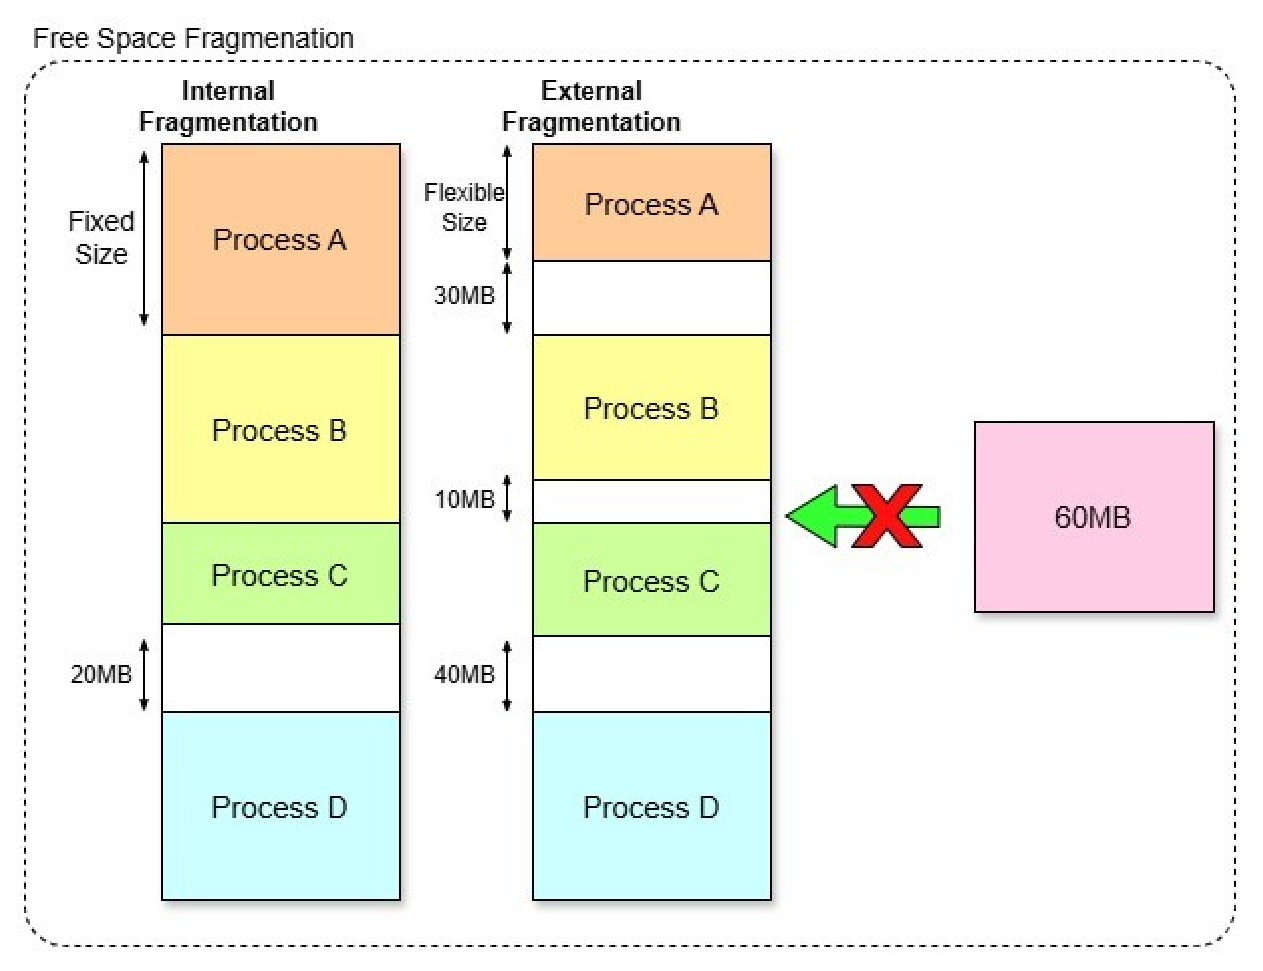
\includegraphics[height=0.25\textheight]{free-fragmentation}
		\label{f:free-fragmentation}
	}
	\hspace{0.5em}
	\subfloat[Data fragmentation] {%
		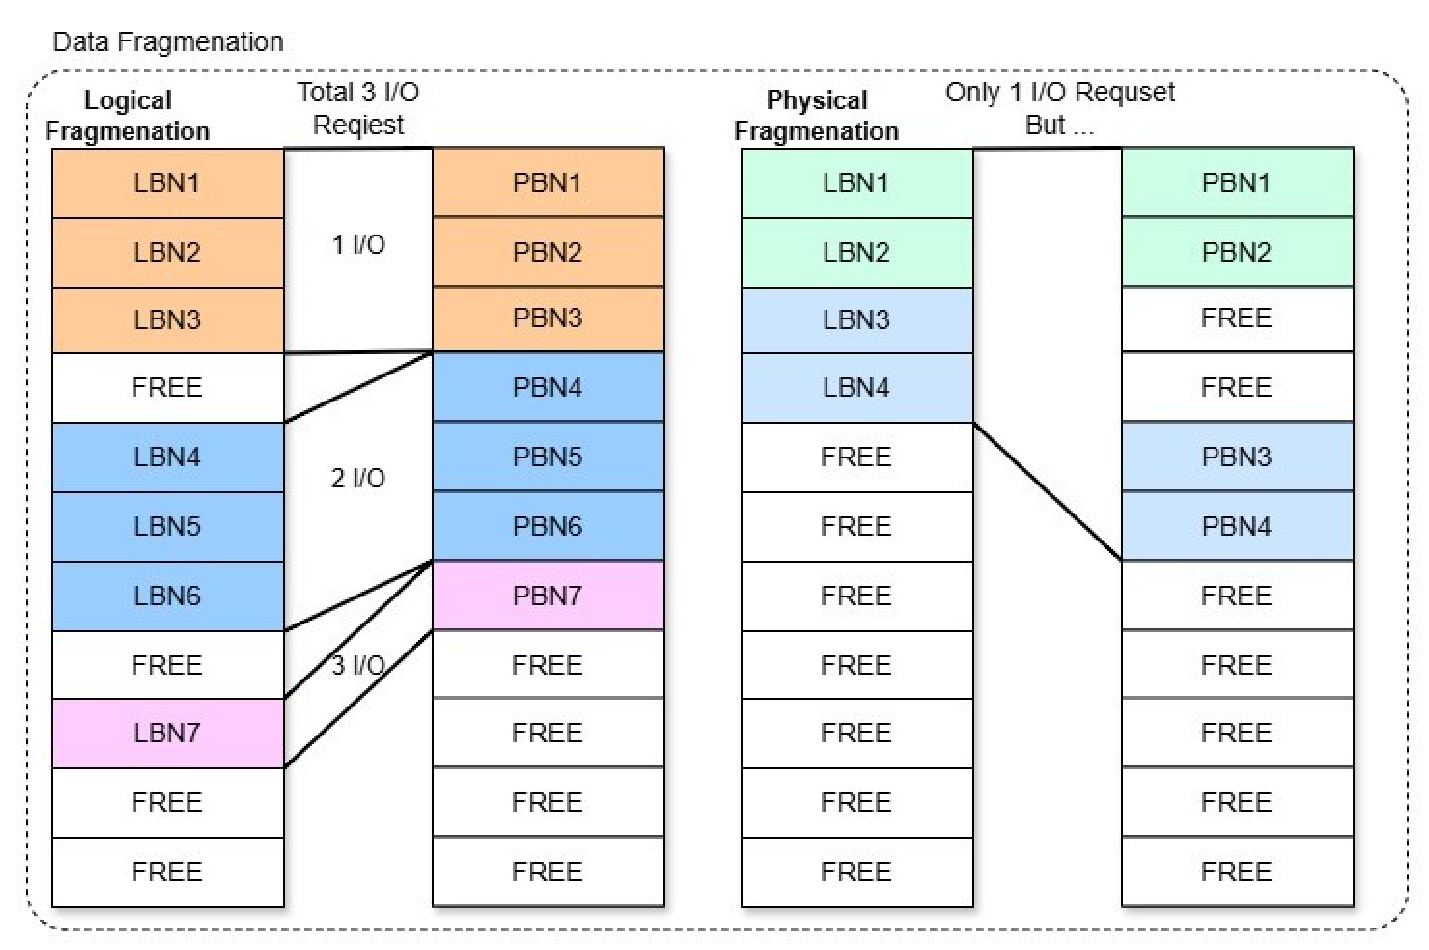
\includegraphics[height=0.25\textheight]{data-fragmentation}
		\label{f:data-fragmentation}
	}
	\caption{Types of fragmentations\label{f:fragmentation}}
\end{figure*}

% Free space fragmentation
Free space fragmentation can be further classified as internal or external fragmentation~\cite{ostep,os-textbook}.
Internal fragmentation occurs when a system employs fixed-size allocation policies, leading to allocated regions containing unused space.
In contrast, external fragmentation occurs when a system repeatedly allocates and deallocates variable-sized chunks.
Through the operations, free space is divided into into small non-contiguous fragments as illustrated in Figure~\ref{f:free-fragmentation}.
This scattered free space makes it difficult to allocate large contiguous blocks, even if the total available free space is sufficient.


% Data fragmentation
Similar to free space, data can be fragmented in computer systems.
In the context of filesystems, data fragmentation occurs when a file is stored in non-contiguous locations in a storage device.
A file may be split into multiple chunks and stored in a fragmented manner.
Notably, data fragmentation can occur even when enough contiguous space is available to store the entire file, due to prior fragmentation or allocation policies.

% Logical fragmentation
As illustrated in Figure~\ref{f:data-fragmentation}, data fragmentation can happen in two forms: \emph{logical fragmentation} and \emph{physical fragmentation}~\cite{janusd:atc17}.
Modern storage devices expose their storage space through logical block addresses~(LBAs), and the host specifies the target data for operations using a starting logical block number~(LBN) and the number of consecutive logical blocks.
Consequently, filesystems must make one I/O request per contiguous LBA chunk.
When a file is fragmented, the filesystem must generate more I/O requests than unfragmented data, thereby experiencing increased interfacing overhead.
Logical fragmentation occurs primarily due to the space allocation policies of filesystems.

% Physical fragmentation
Physical fragmentation originates from the discrepancy between logical and physical address spaces.
Modern storage devices often utilize high-density storage media with complex characteristics and inherent limitations.
Additionally, they typically employ sophisticated data paths and highly parallel architectures for delivering high performance.
As a result, the logical address space exposed to the host does not necessarily align with the physical address space on the storage media and underlying architecture.
Consequently, even if the host issues a single request for a logically contiguous chunk, the device may process it through multiple internal operations.
This is becoming more pronounced in recent devices, where interfacing overhead becomes a non-negligible portion of overall performance~\cite{Problem_in_SSD_Empirical,senescence:fast17,Problem_in_SSD_Mobile_Devices,survey:ictc23,no-afraid:fast24,defrag-mobile:atc17,fragpicker:sosp21}


% Fragmentation matters
In the era of HDDs, fragmentation was a primary source of performance degradation.
The mechanical nature of hard drives means that fragmented files incur significant overhead due to seek time---the delay for moving the disk head to the target track---and rotational delay---the time required for the target sector to rotate under the head.
In contrast, flash memory-based SSDs have no moving parts, eliminating both seek time and rotational delay.
As a result, early research generally assumed that filesystem fragmentation had little to no impact on SSDs.
Moreover, defragmentation was often considered harmful in SSDs, as it generates additional data writes that reduce the lifespan of flash memory~\cite{defrag-mobile:atc17,defrag-lfs:apsys16,parallel-defrag:sac22,Defragmentation_read_collision}.
However, more recent studies have discovered that filesystem aging and the accompanying fragmentation can also degrade SSD performance due to both logical and physical fragmentation~\cite{Problem_in_SSD_Empirical,senescence:fast17,Problem_in_SSD_Mobile_Devices,survey:ictc23,fragpicker:sosp21,no-afraid:fast24}.
For instance, in modern SSDs with complex NAND flash architectures, data may be distributed unevenly across multiple channels and dies.
This imbalance can lead to skewed workloads and reduced I/O parallelism, resulting in suboptimal performance.



%-------------------------------------------------------------------------
\subsection{Flash Translation Layer}\label{ss:ftl}

\begin{comment}
Programs based on the filesystem of a typical operating system recognize disks on a sector basis.
However, in the case of SSDs, storage units are implemented based on pages and blocks.
This means that sector-based programs cannot write directly to SSDs.
Nevertheless, SSDs can easily accommodate these programs because they use the same host interface as HDDs.
To facilitate this, something is needed to assist SSDs in writing for sector-based programs, which is known as the Flash Translation Layer (FTL).

FTL performs two important functions within the SSD: Logical Block Mapping and Garbage Collection (GC).
FTL is responsible for converting logical addresses to physical address values to store logical sectors in physical pages, which is referred to as logical block mapping.
Block mapping is stored in the SSD's memory for quick access and consists of a table containing Logical Block Addresses (LBA) and Physical Block Addresses (PBA).
Additionally, SSDs cannot perform in-place updates.
Therefore, when new data arrives, existing data must be deleted before the new data can be stored.
At this time, the SSD uses GC to preemptively free up space for deleted data, which also contributes to the durability of the SSD.

In this study, we copy and store information from the SSD.
However, accessing the SSD's FTL from the outside is not feasible due to reasons such as security and complexity.
\end{comment}

% Why FTL?
Traditional storage devices, such as hard disk drives (HDDs), interface with the host system through a block-based interface.
This block-based interface abstracts the storage device as a linear array of fixed-size logical sectors.
In contrast, flash memory, which is the medium for solid-state drives (SSDs), is organized into pages and erase blocks.
Data is accessed at the granularity of pages.
However, flash memory imposes a significant constraint.
Once data is written to a page, it cannot be overwritten subsequently.
Instead, the page must be erased before new data can be written.
Moreover, this erase operation can only be performed at the erase block level, which consists of multiple pages.
This erase-before-write constraint, coupled with the mismatch in access units between flash memory and traditional block-based interface, necessitates a translation mechanism in SSDs.
To this end, modern flash-based storage devices, include SSDs, incorporate a firmware layer known as the flash translation layer~(FTL).


% Mapping
The FTL performs two essential functions within an SSD: (1) address mapping and (2) garbage collection~(GC).
The FTL is responsible for translating sector-based logical addresses issued by the host into physical addresses consisting of flash blocks and pages.
To perform the translation, FTL typically maintains a mapping table that is persisted in the flash storage and often cached in volatile memory for fast accesses.

% Garbage collection
The FTL also handles the erase-before-write constraint inherent in flash memory by employing an out-of-place update strategy.
When new data is written, it is placed at a new physical location, and the old data is marked as invalid.
Over time, this process leads to accumulation of invalid data.
When the amount of free space falls below a threshold, the FTL reclaims invalidated space by relocating valid data and erasing blocks.
This process not only recovers space but also contributes to the wear-leveling and overall durability of the SSD.


% Private FTL
Numerous FTL designs have been proposed, each aiming to balance trade-offs among performance, space efficiency, endurance, and implementation complexity~\cite{ftls,ftls,ftls}.
However, SSD manufacturers often make proprietary designs due to concerns related to security and complexity.
As a result, accessing or modifying the FTL from the outside of device is typically infeasible.
This lack of transparency poses challenges for researchers and system developers who seek to understand, optimize, or customize storage behavior.
To address this, several efforts have attempted to expose internal SSD management mechanisms to the host, such as Open-Channel SSDs~\cite{ocssd:fast17}, Zoned Namespace SSDs~\cite{zns:atc21}, and Flexible Data Placement~\cite{fdp}.
Despite these initiatives, the concrete details of FTL implementations and configurations remain largely undisclosed in commercial devices.


%-------------------------------------------------------------------------
\subsection{Related Work}\label{ss:related}

% Fragmentation overview
Many studies have been carried out to investigate the characteristics of fragmentation and its implications for performance~\cite{senescence:fast17,Problem_in_SSD_Empirical,Problem_in_SSD_Mobile_Devices,fsaging:hotstorage19}.
To address the problems caused by fragmentation, there have been investigated two approaches: (1) proactively prevent fragmentation from occurring~\cite{no-afraid:fast24,Defragmentation_read_collision} and (2) defragement already-fragmented data or free space in efficient ways~\cite{defrag-lfs:apsys16,janusd:atc17,fragpicker:sosp21,parallel-defrag:sac22}.


% FragPicker
FragPicker~\cite{fragpicker:sosp21} is a recent study that revisits fragmentation issues in the context of modern storage systems.
The authors demonstrate that fragmentation can indeed lead to performance degradation, even on SSDs.
To address this, FragPicker propses an efficient mechanism to identify hot files by monitoring read and write operations at VFS-level through eBPF.
It than actively deals with the logical fragmentation of these hot files.

% F2FS mobile
Wang et al.~\cite{f2fs-mobile:nvmsa24} investigates how filesystems that employ out-of-place update schemes are prone to fragmentation.
Specifically, in log-structured filesystems, update operations relocate data and it can lead to data fragmentation.
The study Specifically examines F2FS fragmentation on Android mobile devices.
Additionally, the authors propose a scheme to leverage the file-based optimization (FBO) in UFS 4.0~\cite{ufs4.0} to mitigate data fragmetation.


% Fragmentation takes efforts
However, aging filesystems and storage devices is a time-consuming process, often taking days or even longer.
For instance, \cite{fs-aging:sigmetrics97} reports the results of a 3-year study.
Such long-time studies are usually not feasible in many scenarios.
% Preliminary
Accordingly, there has been work attempted to control the preconditioning of filesystems and storage devices.
Earlier studies primarily focused on data fragmentation, where data is scattered across the device.
These studies, however, often neglect the impact of free space fragmentation and its broader implications on filesystem behavior and device aging.

% Geriatrix
Geriatrix~\cite{geriatrix:atc18} is an SSD aging tool that improves upon previous approaches.
It provides a more comprehensive and representative environment for evaluating SSD performance under aged conditions.
Geriatrix addresses earlier limitations by employing a set of built-in aging profiles, which control various parameters such as file size distributions and directory tree depths.
These parameters influence the layout of the filesystem.
The profiles guide the creation and deletion of files in patterns that mimic realistic workloads, thereby effectively reproducing fragmentation characteristics that naturally develop over prolonged usage.
